\section{独立同分布情形}
\label{sec:clt-iid}

标准化部分和$Z_n$的均值和方差已经固定为$0$和$1$，上一节也看到，形状要靠“许多独立的小项”才会变成钟形。最简单的情形是各项来自同一个分布：每一项对总和的贡献都是总方差的$1/n$，没有哪一项占优。本节在这个情形下陈述并证明中心极限定理，只要求方差有限。

\subsection{定理与条件}
\label{sec:clt-iid-theorem}

先看一个偏斜得很厉害的例子。设$X_i\sim\operatorname{Exp}(1)$独立，表示一串相互独立的等待时间，$\mu=\sigma=1$。由第~\ref{chap:random-variable-transformations}章的卷积计算，$S_n\sim\operatorname{Gamma}(n,1)$，所以$Z_n=(S_n-n)/\sqrt{n}$的密度可以精确写出：
\[
 f_{Z_n}(z)=\sqrt{n}\,f_{S_n}(n+z\sqrt{n}),\qquad f_{S_n}(s)=\frac{s^{n-1}\mathrm{e}^{-s}}{(n-1)!}\ (s>0) .
\]
这里用了第~\ref{chap:random-variable-transformations}章的一元换元：$Z_n$是$S_n$的仿射函数，密度要乘以斜率的倒数$\sqrt{n}$。

图~\ref{fig:clt-gamma-densities}画出$n=1,4,16$时的$f_{Z_n}$。$n=1$时它是平移后的指数密度，在$z=-1$处突然跳起，右侧拖着长尾；$n=4$时已经有了圆顶，但峰偏在左边；$n=16$时与标准高斯密度只差一点偏斜。偏斜的程度可以用偏度衡量，$\operatorname{Gamma}(n,1)$的偏度是$2/\sqrt{n}$，按$1/\sqrt{n}$消失。

\begin{BookInlineFigure}
 \centering
 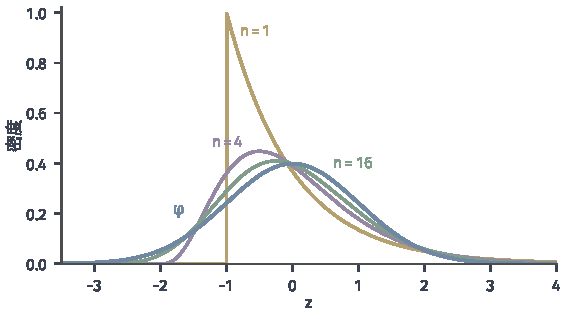
\includegraphics[width=96mm]{figures/07-probability/03-probability-limits/matplotlib/clt-gamma-densities/figure.pdf}
 \caption{$n$个独立$\operatorname{Exp}(1)$之和的标准化$Z_n=(S_n-n)/\sqrt{n}$的精确密度，$n=1$（黄）、$4$（紫）、$16$（绿），蓝线为标准高斯密度$\varphi$。$n=1$时密度在$z=-1$处从$0$跳到$1$。}
 \label{fig:clt-gamma-densities}
\end{BookInlineFigure}

硬币与等待时间的单项分布截然不同，一个只取两个值，一个是连续的偏斜密度，标准化和却都趋于同一个形状。下面的定理说，只要独立、同分布、方差有限且为正，这个现象总会发生。

\begin{theorem}[独立同分布的中心极限定理]
\label{thm:clt-iid}
设$X_1,X_2,\dots$独立同分布，$\mathbb{E}[X_1]=\mu$，$\operatorname{Var}(X_1)=\sigma^2\in(0,\infty)$，$Z_n$如式~\eqref{eq:clt-zn}。则
\begin{equation}
 Z_n=\frac{S_n-n\mu}{\sigma\sqrt{n}}\xrightarrow{\mathrm{d}}\mathcal{N}(0,1) .
 \label{eq:clt-iid}
\end{equation}
\end{theorem}

\paragraph{用分布函数表述}
标准高斯分布函数$\Phi$处处连续，没有需要排除的跳点。由第~\ref{chap:weak-convergence-of-distributions}章的分布函数判据，式~\eqref{eq:clt-iid}等价于对每个实数$x$，
\begin{equation}
 \mathbb{P}(Z_n\leq x)\to\Phi(x) .
 \label{eq:clt-iid-cdf}
\end{equation}
于是对任意$a<b$，$\mathbb{P}(a<Z_n\leq b)\to\Phi(b)-\Phi(a)$。端点是否取等号不影响极限：$\mathbb{P}(Z_n=x)\leq\mathbb{P}(x-\eta<Z_n\leq x)$对每个$\eta>0$成立，右边趋于$\Phi(x)-\Phi(x-\eta)$，可以任意小。

把定理用于$X_i\sim\operatorname{Bern}(p)$，$0<p<1$，就得到二项计数的正态逼近：
\[
 \frac{S_n-np}{\sqrt{np(1-p)}}\xrightarrow{\mathrm{d}}\mathcal{N}(0,1),\qquad S_n\sim\operatorname{Bin}(n,p) .
\]
这个特例称为\term{de Moivre--Laplace定理}（de Moivre--Laplace theorem），它是中心极限定理最早的形式。

\paragraph{各个条件的作用}
定理有三个条件。独立性使和的特征函数能拆成乘积，这是证明的起点；同分布使每个因子相同，$n$个小贡献完全对称；方差有限且为正，既给出了标准化的尺度，也保证下面的二阶展开成立。上一节的特制硬币各项分布随$n$变化，不在定理的范围里，它的极限也确实不是高斯的。

定理只要求二阶矩有限，不要求三阶矩，也不要求矩母函数存在。第~\ref{sec:clt-error}节估计近似误差时要用三阶绝对矩，那是为了得到收敛的速度，不是收敛本身的条件。第~\ref{chap:weak-convergence-of-distributions}章说明过，矩母函数可能在零点附近的任何邻域都无穷，而特征函数总是存在，所以证明用特征函数。

\subsection{特征函数证明}
\label{sec:clt-iid-proof}

把$X_i$标准化，令$Y_i=(X_i-\mu)/\sigma$。$Y_i$独立同分布，$\mathbb{E}[Y_i]=0$，$\mathbb{E}[Y_i^2]=1$，并且
\[
 Z_n=\frac{1}{\sqrt{n}}\sum_{i=1}^{n}Y_i .
\]
记$Y$为与$Y_i$同分布的变量，$\phi_Y$为它的特征函数。第~\ref{chap:weak-convergence-of-distributions}章给出了两条运算规则：数乘满足$\phi_{cY}(t)=\phi_Y(ct)$；独立变量之和的特征函数是各自特征函数的乘积。合起来，
\begin{equation}
 \phi_{Z_n}(t)=\prod_{i=1}^{n}\phi_{Y_i}\Bigl(\frac{t}{\sqrt{n}}\Bigr)=\phi_Y\Bigl(\frac{t}{\sqrt{n}}\Bigr)^{n} .
 \label{eq:clt-product}
\end{equation}
标准高斯分布的特征函数是$\mathrm{e}^{-t^2/2}$，由连续性定理，只需证明式~\eqref{eq:clt-product}对每个$t$趋于$\mathrm{e}^{-t^2/2}$。

\paragraph{为什么会出现$\mathrm{e}^{-t^2/2}$}
先用直觉看一遍。$t/\sqrt{n}$很小，$\phi_Y$在原点附近的展开是
\[
 \phi_Y(s)=\mathbb{E}[\mathrm{e}^{\mathrm{i}sY}]\approx1+\mathrm{i}s\,\mathbb{E}[Y]-\frac{s^2}{2}\mathbb{E}[Y^2]=1-\frac{s^2}{2} .
\]
代入$s=t/\sqrt{n}$再取$n$次方，
\[
 \phi_{Z_n}(t)\approx\Bigl(1-\frac{t^2}{2n}\Bigr)^{n}\to\mathrm{e}^{-t^2/2} .
\]
中心化让一次项消失，方差为一让二次项的系数是$1/2$。剩下要说明的是：被“$\approx$”丢掉的余项乘上$n$个因子以后，累计起来仍然可以忽略。

第~\ref{chap:weak-convergence-of-distributions}章在二阶矩有限时给出了上面的展开，余项是$s^2$的高阶无穷小。为了在$n$个因子的乘积里累计余项，我们把余项写成显式的界，下面两个引理分别处理单个因子和乘积。

\begin{lemma}[复指数的二阶展开]
\label{lem:clt-exp-remainder}
对每个实数$x$，
\begin{equation}
 \Bigl\lvert\mathrm{e}^{\mathrm{i}x}-1-\mathrm{i}x+\frac{x^2}{2}\Bigr\rvert\leq\min\Bigl\{\frac{\lvert x\rvert^{3}}{6},\ x^2\Bigr\} .
 \label{eq:clt-exp-remainder}
\end{equation}
\end{lemma}

\begin{proof}
对积分$\int_0^x(x-u)\mathrm{e}^{\mathrm{i}u}\,\mathrm{d}u$分部积分，取$\mathrm{e}^{\mathrm{i}u}$的原函数$-\mathrm{i}\mathrm{e}^{\mathrm{i}u}$，得到
\[
 \int_0^x(x-u)\mathrm{e}^{\mathrm{i}u}\,\mathrm{d}u
 =\Bigl[-\mathrm{i}(x-u)\mathrm{e}^{\mathrm{i}u}\Bigr]_0^x-\mathrm{i}\int_0^x\mathrm{e}^{\mathrm{i}u}\,\mathrm{d}u
 =\mathrm{i}x-(\mathrm{e}^{\mathrm{i}x}-1) .
\]
移项得到一次展开的余项公式
\[
 \mathrm{e}^{\mathrm{i}x}-1-\mathrm{i}x=-\int_0^x(x-u)\mathrm{e}^{\mathrm{i}u}\,\mathrm{d}u .
\]

第一个界。$x^2/2=\int_0^x(x-u)\,\mathrm{d}u$，与上式相加，
\[
 \mathrm{e}^{\mathrm{i}x}-1-\mathrm{i}x+\frac{x^2}{2}=\int_0^x(x-u)\bigl(1-\mathrm{e}^{\mathrm{i}u}\bigr)\,\mathrm{d}u .
\]
被积函数中$\lvert1-\mathrm{e}^{\mathrm{i}u}\rvert\leq2$，$x-u$在积分区间上不变号，所以
\[
 \Bigl\lvert\mathrm{e}^{\mathrm{i}x}-1-\mathrm{i}x+\frac{x^2}{2}\Bigr\rvert\leq2\Bigl\lvert\int_0^x(x-u)\,\mathrm{d}u\Bigr\rvert=x^2 .
\]

第二个界。再对$\int_0^x(x-u)^2\mathrm{e}^{\mathrm{i}u}\,\mathrm{d}u$分部积分，并代入前面的结果：
\[
 \int_0^x(x-u)^2\mathrm{e}^{\mathrm{i}u}\,\mathrm{d}u
 =\mathrm{i}x^2-2\mathrm{i}\int_0^x(x-u)\mathrm{e}^{\mathrm{i}u}\,\mathrm{d}u
 =\mathrm{i}x^2-2\mathrm{i}\bigl(1+\mathrm{i}x-\mathrm{e}^{\mathrm{i}x}\bigr) .
\]
两边除以$2\mathrm{i}$并整理，
\[
 \mathrm{e}^{\mathrm{i}x}-1-\mathrm{i}x+\frac{x^2}{2}=\frac{1}{2\mathrm{i}}\int_0^x(x-u)^2\mathrm{e}^{\mathrm{i}u}\,\mathrm{d}u .
\]
被积函数的模是$(x-u)^2$，所以
\[
 \Bigl\lvert\mathrm{e}^{\mathrm{i}x}-1-\mathrm{i}x+\frac{x^2}{2}\Bigr\rvert\leq\frac12\Bigl\lvert\int_0^x(x-u)^2\,\mathrm{d}u\Bigr\rvert=\frac{\lvert x\rvert^3}{6} .
\]
\end{proof}

两个界各管一段，见图~\ref{fig:clt-remainder}。$\lvert x\rvert$小的时候，三次界$\lvert x\rvert^3/6$更小，余项确实是三阶小量；$\lvert x\rvert$大的时候，二次界$x^2$更小，因为余项最多和$x^2/2$同阶，不会像$\lvert x\rvert^3$那样增长。两条界在$\lvert x\rvert=6$处相交。证明中正是要用后一个界：$Y$只有二阶矩，$\mathbb{E}[\lvert Y\rvert^3]$可能是无穷，但$\mathbb{E}[Y^2]$一定有限。

\begin{BookInlineFigure}
 \centering
 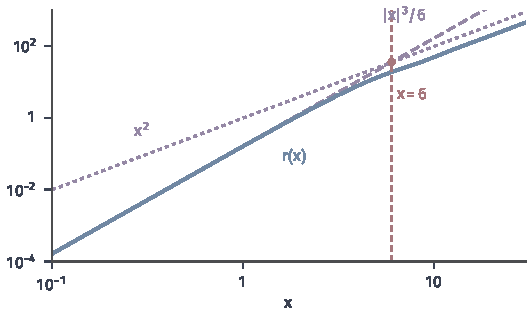
\includegraphics[width=90mm]{figures/07-probability/03-probability-limits/matplotlib/clt-remainder/figure.pdf}
 \caption{二阶展开的余项$r(x)=\lvert\mathrm{e}^{\mathrm{i}x}-1-\mathrm{i}x+x^2/2\rvert$（蓝）与两条上界$\lvert x\rvert^3/6$（紫色虚线）、$x^2$（紫色点线），双对数坐标。两条界在$x=6$（红点）相交，$x<6$时三次界更紧，$x>6$时二次界更紧。}
 \label{fig:clt-remainder}
\end{BookInlineFigure}

\begin{lemma}[乘积之差]
\label{lem:clt-product-difference}
设复数$z_1,\dots,z_m$与$w_1,\dots,w_m$的模都不超过$1$。则
\begin{equation}
 \Bigl\lvert\prod_{k=1}^{m}z_k-\prod_{k=1}^{m}w_k\Bigr\rvert\leq\sum_{k=1}^{m}\lvert z_k-w_k\rvert .
 \label{eq:clt-product-difference}
\end{equation}
\end{lemma}

\begin{proof}
对$m$归纳。$m=1$时两边相等。设结论对$m-1$成立，记$P=\prod_{k<m}z_k$，$Q=\prod_{k<m}w_k$，它们的模不超过$1$。拆开差，
\[
 Pz_m-Qw_m=z_m(P-Q)+(z_m-w_m)Q .
\]
由$\lvert z_m\rvert\leq1$与$\lvert Q\rvert\leq1$，
\[
 \lvert Pz_m-Qw_m\rvert\leq\lvert P-Q\rvert+\lvert z_m-w_m\rvert ,
\]
再对$\lvert P-Q\rvert$用归纳假设即得。
\end{proof}

这个引理说，模不超过一的因子相乘时，各因子的误差至多简单相加，不会被放大。所以只要每个因子的误差是$o(1/n)$，$n$个因子的累计误差就是$o(1)$。

\begin{proof}[定理~\ref{thm:clt-iid}的证明]
固定$t$，记$s=t/\sqrt{n}$。

第一步，单个因子的误差。在式~\eqref{eq:clt-exp-remainder}中令$x=sY$，取期望。由$\mathbb{E}[Y]=0$，$\mathbb{E}[Y^2]=1$，左边期望里的各项分别给出$\phi_Y(s)$、$1$、$0$和$s^2/2$；再用“期望的模不超过模的期望”，得到
\[
 \Bigl\lvert\phi_Y(s)-\Bigl(1-\frac{s^2}{2}\Bigr)\Bigr\rvert
 \leq\mathbb{E}\Bigl[\min\Bigl\{\frac{\lvert s\rvert^{3}\lvert Y\rvert^{3}}{6},\ s^2Y^2\Bigr\}\Bigr] .
\]
代入$s=t/\sqrt{n}$，两边乘$n$，
\[
 n\Bigl\lvert\phi_Y\Bigl(\frac{t}{\sqrt{n}}\Bigr)-\Bigl(1-\frac{t^2}{2n}\Bigr)\Bigr\rvert
 \leq t^2\,\mathbb{E}\Bigl[\min\Bigl\{\frac{\lvert t\rvert\,\lvert Y\rvert^{3}}{6\sqrt{n}},\ Y^2\Bigr\}\Bigr] .
\]

第二步，右边趋于零。期望里的随机变量对每个样本点都趋于零，因为$\lvert Y\rvert^3/\sqrt{n}\to0$；它又被可积的$Y^2$控制。由支配收敛定理，右边的期望趋于零。这里只用到$\mathbb{E}[Y^2]<\infty$。

第三步，累计。$n\geq t^2/2$时，$\lvert1-t^2/(2n)\rvert\leq1$；特征函数的模也不超过$1$。对式~\eqref{eq:clt-product}的$n$个因子用引理~\ref{lem:clt-product-difference}，
\[
 \Bigl\lvert\phi_{Z_n}(t)-\Bigl(1-\frac{t^2}{2n}\Bigr)^{n}\Bigr\rvert
 \leq n\Bigl\lvert\phi_Y\Bigl(\frac{t}{\sqrt{n}}\Bigr)-\Bigl(1-\frac{t^2}{2n}\Bigr)\Bigr\rvert\to0 .
\]

第四步，极限。由$\ln(1-y)/y\to-1$（$y\to0$），$n\ln(1-t^2/(2n))\to-t^2/2$，所以
\[
 \Bigl(1-\frac{t^2}{2n}\Bigr)^{n}\to\mathrm{e}^{-t^2/2} .
\]
两步合起来，$\phi_{Z_n}(t)\to\mathrm{e}^{-t^2/2}$对每个$t$成立。极限是$\mathcal{N}(0,1)$的特征函数，由连续性定理，$Z_n\xrightarrow{\mathrm{d}}\mathcal{N}(0,1)$。
\end{proof}

图~\ref{fig:clt-proof-flow}把证明的链条和每一环所用的条件放在一起。独立性只在第一个方框用到；中心化和方差为一决定展开式的形状；二阶矩有限只在支配收敛那一步用到；最后由连续性定理从特征函数回到分布。

\begin{BookInlineFigure}
 \centering
 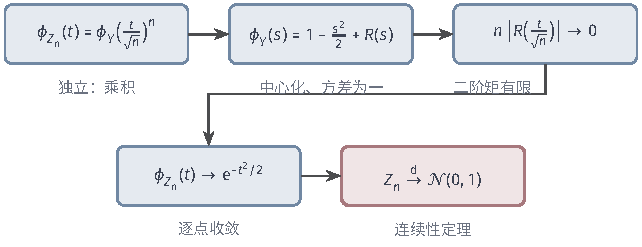
\includegraphics[width=109mm]{figures/07-probability/03-probability-limits/tikz/clt-proof-flow/figure.pdf}
 \caption{中心极限定理的特征函数证明。方框是各步得到的结论，框下灰字是该步所用的条件或工具，红框是要证明的依分布收敛。}
 \label{fig:clt-proof-flow}
\end{BookInlineFigure}

\paragraph{去掉中心化会怎样}
若不减去$\mu$，直接看$S_n/(\sigma\sqrt{n})$，它的特征函数多出因子$\mathrm{e}^{\mathrm{i}t\sqrt{n}\mu/\sigma}$。$\mu\neq0$时这个因子绕单位圆越转越快，对$t\neq0$没有极限，分布的位置以$\sqrt{n}$的速度跑向无穷。中心化就是把这个漂移去掉。

\paragraph{硬币的特征函数}
用硬币核对一遍。把一次结果写成$Y=2X-1$，以各$1/2$的概率取$\pm1$，它已经中心化且方差为一。它的特征函数是
\[
 \phi_Y(s)=\tfrac12\mathrm{e}^{\mathrm{i}s}+\tfrac12\mathrm{e}^{-\mathrm{i}s}=\cos s .
\]
由式~\eqref{eq:clt-product}，$\phi_{Z_n}(t)=\cos(t/\sqrt{n})^{n}$。取$t=1$，$n=1,4,16$时依次为
\[
 \cos1\approx0.5403,\qquad \cos(0.5)^{4}\approx0.5931,\qquad \cos(0.25)^{16}\approx0.6033 ,
\]
极限值是$\mathrm{e}^{-1/2}\approx0.6065$。$n=16$时，近似式$(1-t^2/(2n))^n=(1-1/32)^{16}\approx0.6017$也已接近极限。

证明中的几个量也可以在这里逐一算出。$n=16$、$t=1$时$s=1/4$，单个因子的误差是
\[
 \Bigl\lvert\cos\frac14-\Bigl(1-\frac{1}{32}\Bigr)\Bigr\rvert\approx\lvert0.968912-0.968750\rvert\approx1.62\times10^{-4} ,
\]
乘以$n=16$得到约$2.6\times10^{-3}$。第三步说两个乘积之差不超过这个数，实际的差是
\[
 \lvert0.6033-0.6017\rvert\approx1.6\times10^{-3} .
\]
第一步的上界中$\lvert Y\rvert=1$，它给出
\[
 t^2\,\mathbb{E}\Bigl[\min\Bigl\{\frac{\lvert t\rvert\,\lvert Y\rvert^{3}}{6\sqrt{n}},\ Y^2\Bigr\}\Bigr]=\frac{1}{24}\approx0.042 ,
\]
比实际误差大得多。原因是硬币对称，$\mathbb{E}[Y^3]=0$，$\cos s$的展开中没有三次项，误差从四次项$s^4/24$开始；引理~\ref{lem:clt-exp-remainder}不知道这种对称性，只能按三次估计。证明只需要误差趋于零，不需要它紧。

图~\ref{fig:clt-charfun-convergence}(a)画出整条曲线。$n=1$时$\cos t$在$t=\pm\pi$处等于$-1$，周期地回到$1$，这反映硬币只取格点值；$n$增大时，第一个回到$1$的位置$t=\pi\sqrt{n}$被推向远处，中间部分贴上$\mathrm{e}^{-t^2/2}$。收敛是逐点的，不是在整条实轴上一致的：$t=\pi\sqrt{n}$处总有$\lvert\phi_{Z_n}\rvert=1$。连续性定理只需要逐点收敛。图~\ref{fig:clt-charfun-convergence}(b)是指数等待时间的情形，特征函数取复值，画的是实部，它从一开始就向零衰减，几项以后就与高斯曲线难以区分。

\begin{BookInlineFigure}
 \centering
 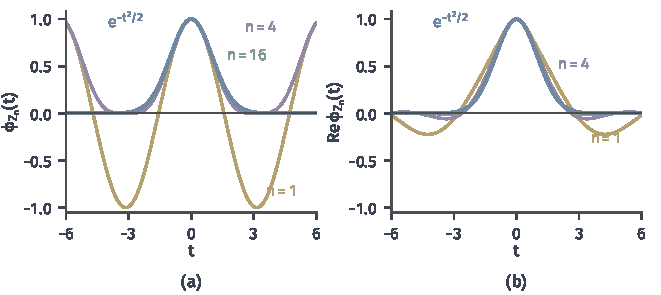
\includegraphics[width=112mm]{figures/07-probability/03-probability-limits/matplotlib/clt-charfun-convergence/figure.pdf}
 \caption{标准化和的特征函数与$\mathrm{e}^{-t^2/2}$（蓝）的比较，$n=1$（黄）、$4$（紫）、$16$（绿；与蓝线几乎重合）。(a)$\pm1$等可能的硬币，$\phi_{Z_n}(t)=\cos(t/\sqrt{n})^{n}$；(b)$\operatorname{Exp}(1)$等待时间，$\phi_{Z_n}(t)=\mathrm{e}^{-\mathrm{i}t\sqrt{n}}(1-\mathrm{i}t/\sqrt{n})^{-n}$的实部。}
 \label{fig:clt-charfun-convergence}
\end{BookInlineFigure}

\subsection{样本平均的正态近似}
\label{sec:clt-sample-mean}

实际使用时，人们关心的是$\bar{X}_n$落在某个区间的概率。把$Z_n\leq x$改写成$\bar{X}_n\leq\mu+x\sigma/\sqrt{n}$，式~\eqref{eq:clt-iid-cdf}就是
\begin{equation}
 \mathbb{P}\Bigl(\bar{X}_n\leq\mu+\frac{x\sigma}{\sqrt{n}}\Bigr)\to\Phi(x),\qquad x\in\mathbb{R} .
 \label{eq:clt-sample-mean}
\end{equation}
人们常把它简写成$\bar{X}_n\approx\mathcal{N}(\mu,\sigma^2/n)$。这个记号的含义是：在$\mu$附近、以$\sigma/\sqrt{n}$为单位量出的阈值上，$\bar{X}_n$的分布函数接近相应的高斯分布函数。

近似的中心是总体均值$\mu$，尺度是$\sigma/\sqrt{n}$，两者都要对。中心取错一个固定量$c$，以$\sigma/\sqrt{n}$为单位就差了$c\sqrt{n}/\sigma$个单位，$n$越大错得越远；尺度用$\sigma/n$或$\sigma$，就回到了第~\ref{sec:clt-scales}节中$a\neq1/2$的情形。

\paragraph{高斯样本：精确}
若$X_i\sim\mathcal{N}(\mu,\sigma^2)$独立，第~\ref{chap:multivariate-distributions}章的线性组合公式给出，对每个$n$，
\[
 \bar{X}_n\sim\mathcal{N}\Bigl(\mu,\frac{\sigma^2}{n}\Bigr),\qquad Z_n\sim\mathcal{N}(0,1) .
\]
这时式~\eqref{eq:clt-sample-mean}左边恒等于$\Phi(x)$，不需要取极限。对一般的样本，式~\eqref{eq:clt-sample-mean}只是$n\to\infty$时的结论，它本身不告诉我们在$n=20$或$n=100$时误差有多大。

\paragraph{二项计数}
设$S\sim\operatorname{Bin}(20,0.3)$，则$np=6$，$np(1-p)=4.2$。精确地，
\[
 \mathbb{P}(S\leq8)\approx0.8867 .
\]
直接套用$\mathcal{N}(6,4.2)$，
\[
 \Phi\Bigl(\frac{8-6}{\sqrt{4.2}}\Bigr)=\Phi(0.976)\approx0.8354 ,
\]
差了约$0.05$。

误差的一个来源是$S$只取整数。$\mathbb{P}(S\leq8)$和$\mathbb{P}(S<9)$是同一个数，阈值在$[8,9)$内任意移动，左边都不变，高斯分布函数却在这一段上从$0.835$升到$0.928$。取中点$8.5$作为阈值，
\[
 \Phi\Bigl(\frac{8.5-6}{\sqrt{4.2}}\Bigr)=\Phi(1.220)\approx0.8887 ,
\]
误差降到$0.002$。这种做法称为\term{连续性修正}（continuity correction）。章首的硬币也一样：$\mathbb{P}(S_{100}\leq55)\approx0.8644$，不修正的近似值是$\Phi(1)\approx0.8413$，修正后是$\Phi(1.1)\approx0.8643$。

图~\ref{fig:clt-binomial-cdf}画出$\operatorname{Bin}(20,0.3)$的分布函数阶梯和两条高斯曲线。不修正的蓝线大致在每级台阶的中点处达到台阶的高度，在整数阈值处偏低；修正后的黄线整体左移半格，在台阶的左端点，也就是整数阈值处，与阶梯的高度相合。连续性修正只是格点分布上的一个经验做法，它不改变极限，也不提供误差保证；有保证的误差界在第~\ref{sec:clt-error}节给出。

\begin{BookInlineFigure}
 \centering
 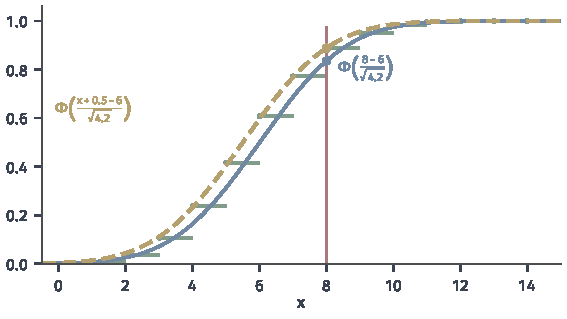
\includegraphics[width=96mm]{figures/07-probability/03-probability-limits/matplotlib/clt-binomial-cdf/figure.pdf}
 \caption{$S\sim\operatorname{Bin}(20,0.3)$的分布函数（绿色阶梯）、高斯近似$\Phi((x-6)/\sqrt{4.2})$（蓝）与连续性修正后的$\Phi((x+0.5-6)/\sqrt{4.2})$（黄色虚线）。红线标出阈值$8$，三点依次为精确值$0.8867$、修正值$0.8887$与未修正值$0.8354$。}
 \label{fig:clt-binomial-cdf}
\end{BookInlineFigure}

\paragraph{需要掷多少次}
正态近似也可以反过来用：给定精度，估计所需的样本量。要使硬币的正面比例与$1/2$相差不超过$0.01$的概率约为$0.95$，由式~\eqref{eq:clt-sample-mean}，需要$0.01$约等于$1.96$个$\sigma/\sqrt{n}$，其中$1.96$是标准高斯分布的$97.5\%$分位数。代入$\sigma=1/2$，
\[
 1.96\cdot\frac{1/2}{\sqrt{n}}=0.01,\qquad n=\Bigl(\frac{1.96\times0.5}{0.01}\Bigr)^2=9604 .
\]

用第~\ref{chap:tail-probabilities}章的Chebyshev不等式也能回答这个问题，而且答案有保证：要使比例偏离$1/2$至少$0.01$的概率不超过$0.05$，只需
\[
 \frac{\sigma^2}{n\cdot0.01^2}=\frac{0.25}{0.0001\,n}\leq0.05,\qquad n\geq50000 .
\]
两个答案相差五倍多。Chebyshev不等式对一切方差为$1/4$的分布都成立，所以保守；正态近似利用了“和接近高斯”这一额外信息，所以省得多，但它只是近似。$n=9604$时这个近似有多准，要等第~\ref{sec:clt-error}节的误差界来回答。

\paragraph{偏斜样本}
指数等待时间没有格点问题，误差来自偏斜。$n=10$时，平均等待时间不超过均值$1$的概率是
\[
 \mathbb{P}(\bar{X}_{10}\leq1)=\mathbb{P}(S_{10}\leq10)\approx0.5421 ,
\]
而式~\eqref{eq:clt-sample-mean}给出$\Phi(0)=0.5$。右偏的分布把中位数拉到均值左边，均值处的分布函数值因此超过$1/2$。图~\ref{fig:clt-gamma-densities}中$n=16$的密度峰仍略偏左，是同一现象。
